\section{Pilot Study}

The ai

\subsection{Methodology}

The methodology set out above was implemented in five different Central London locations at different times.
\% Sensors were installed and data collected for extended periods of time.
Sensors were installed and data collected for extended periods of time.

We then applied the methodologies discussed earlier to arrive at estimated pedestrian footfall and compared them with the corresponding manual counts.
We finally evaluated the effectiveness of the processes with the Mean Absolute Percentage Error (MAPE) at the locations and report our findings below.


\subsection{Locations}

\begin{figure}
  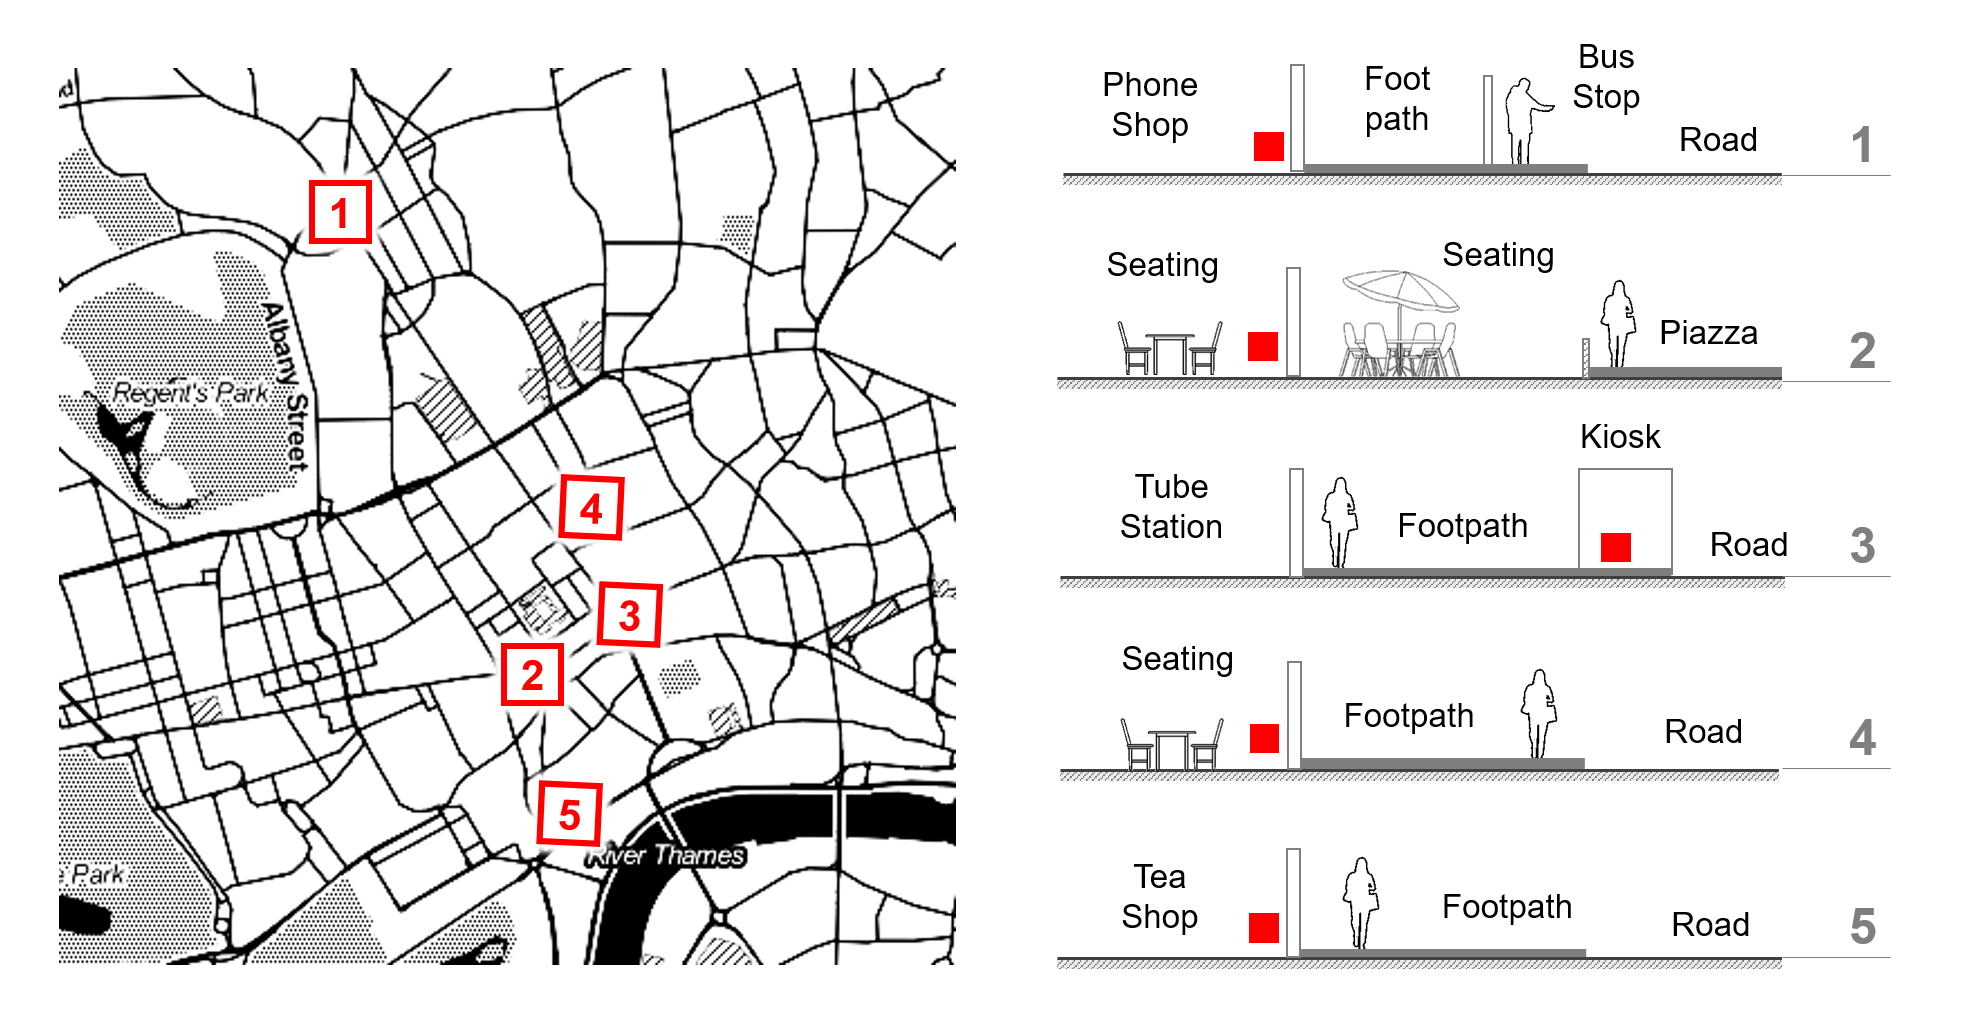
\includegraphics[trim={20 20 20 20},clip]{images/pilot-study-locations.png}
  \caption{Outline of the `Medium data toolkit' devised to collect, process, visualise and manage the Wi-Fi probe requests data}
  \label{figure:literature:tech:timeline}
\end{figure}

Locations where sensors were installed, volume and speed of probe requests collected by the sensor and total pedestrians manually counted.
The data occupies around 1.8 GB on disk when encoded in text format.
The locations at which the data were collected are shown in Table .
The locations were chosen for their diverse site conditions and unique sources of noise around the potential location of the sensors.
The position of the sensor at these locations with respect to the context is shown the Figure 
We can see that Location 5 is the `cleanest' with one clear stationary source of noise (phone shop) while location 2 is the most complex due to the proximity of seating areas to the sensor.
The sensors were operational through out February and March, while manual counts were conducted in these locations in half hour sessions on at least two different days.
For the purposes of comparing with ground truth, we considered the data from sensors which correspond to the 12 sets of available manual counts.
The schedule of data collection is shown in Figure .

\begin{figure*}
  
\includegraphics{images/pilot-study-schedule.png}
  \caption{Outline of the `Medium data toolkit' devised to collect, process, visualise and manage the Wi-Fi probe requests data}
  \label{figure:literature:tech:timeline}
\end{figure*}


\begin{table}
  \footnotesize
  \begin{center}
    \begin{tabular}{cm{2.5cm}lm{2.3cm}m{1.5cm}m{1.5cm}}
      \toprule
        ID & Location & Type & Installation notes & Probe Requests & Counted Footfall\\
      \midrule
        \addlinespace[0.4cm]
        1 & Camden High Street & Phone Shop & Bus stop in front & 9.9 (297) & 3683 (33)\\
        \addlinespace[0.2cm]
        2 & Central St.Giles & Restaurant & Seating area on both sides & 3.9 (169) & 0346 (05)\\
        \addlinespace[0.2cm]
        3 & Holborn Station & Info. Kiosk & Overlooks station entrance & 4.3 (303) & 2956 (46)\\
        \addlinespace[0.2cm]
        4 & Brunswick Center & Fast Food & Has seating area on one side & 3.4 (210) & 0960 (12)\\
        \addlinespace[0.2cm]
        5 & The Strand & Tea Shop & Phone shop next door & 8.4 (382) & 1969 (21)\\
        \addlinespace[0.1cm]
      \bottomrule
    \end{tabular}
  \end{center}
  \caption{Locations of installed sensors}
  \label{table:collection:pilot:location}
\end{table}

\subsection{Data Collection}



